\documentclass{zettel}

%\renewcommand{\gregor}{\put(10.0,-3.5){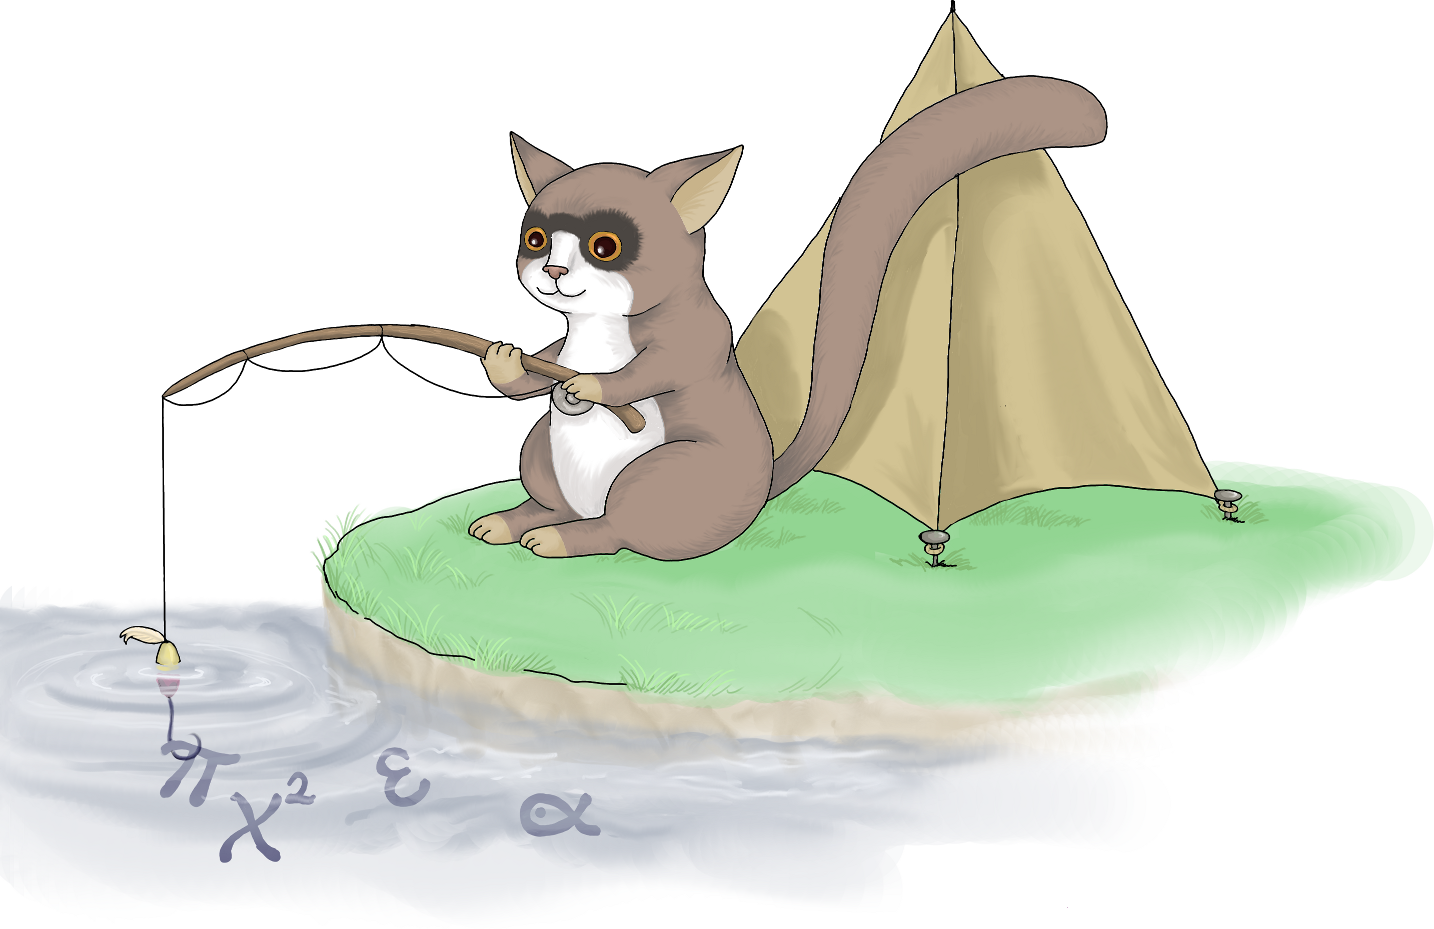
\includegraphics[scale=0.18]{campgregor}}}

\usepackage{framed}
\definecolor{shadecolor}{rgb}{.97,.97,.97}
\begin{document}

\renewcommand{\betreff}{Mathecamp des Matheschülerzirkels Augsburg vom 16. bis
20. August}

\makeletterhead{}
\begin{picture}(0,0)
  \put(9,-19){%
    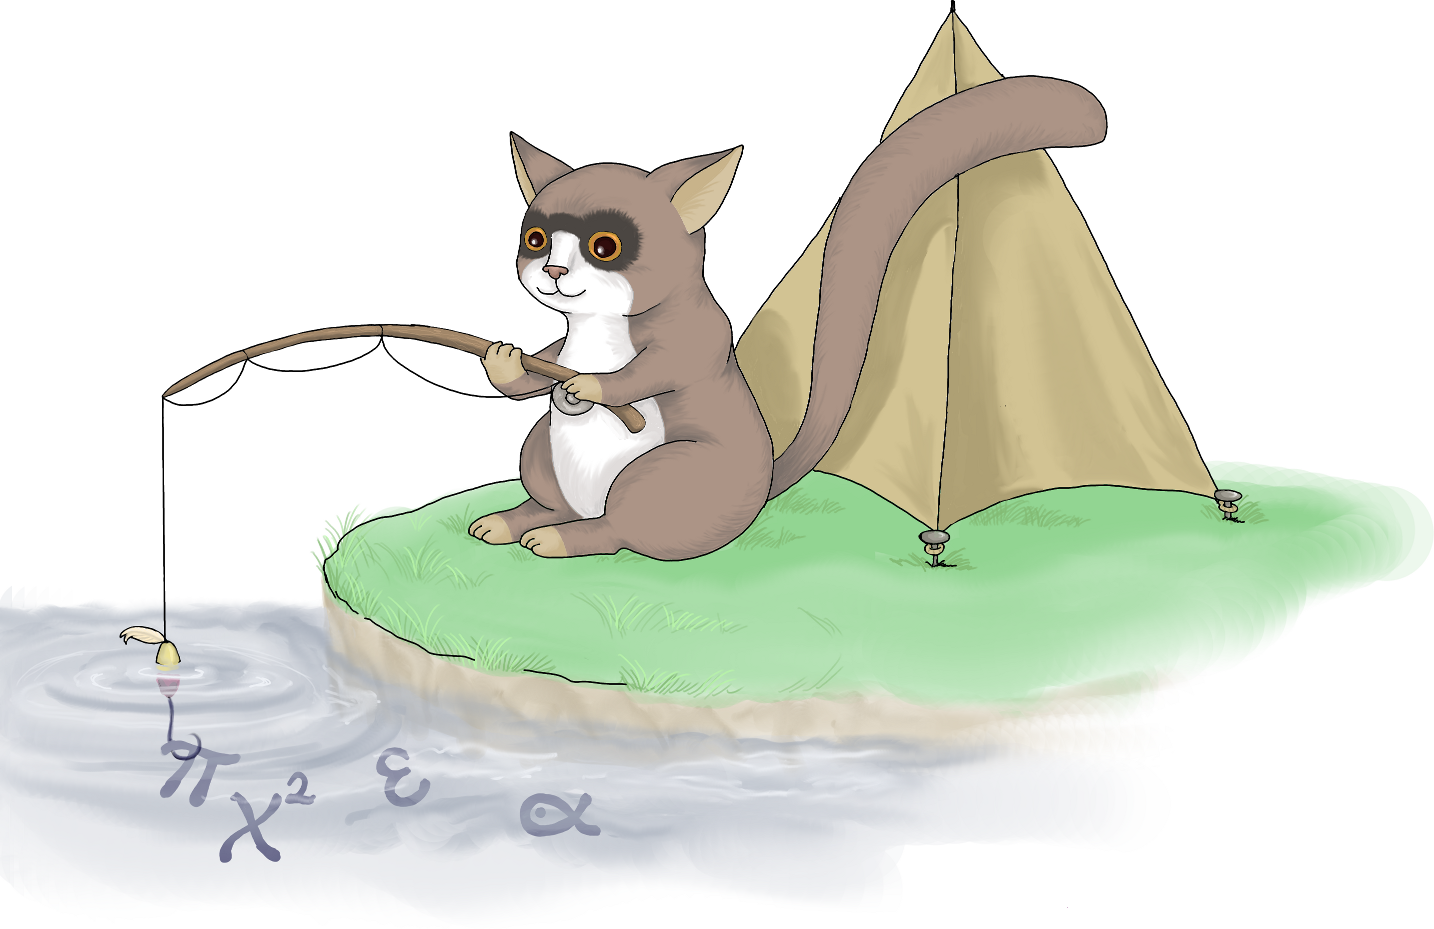
\includegraphics[scale=0.2]{campgregor}
  }
\end{picture}
\vspace{-2em}

Liebe Schülerinnen und Schüler, liebe Eltern,

wir laden euch herzlich zum ersten Mathecamp des Matheschülerzirkels Augsburg
ein. Dort werden wir mit euch tolle mathematische Themen verstehen und die
Freizeit in den Ferien genießen.

\begin{tabbing}
  \hspace{2.2cm} \= \kill
  \textbf{Was?} \> Mathematik und Spaß in den Ferien \\
  \textbf{Wann?} \> 16. bis 20. August 2014 (Samstag bis Mittwoch) \\
  \textbf{Wo?} \> Bruder-Klaus-Heim in Violau (St. Michael Straße 15, 86450 Violau) \\
  \textbf{Für wen?} \> \begin{minipage}[t]{\dimexpr\textwidth-2.3cm}
  Einzige Teilnahmevoraussetzung ist Spaß und Interesse an
  Mathematik.
  Jeder kann mitkommen, auch, wenn man nicht bei den Zirkeln
  mitgemacht hat.\end{minipage} \\
  \textbf{Kosten?} \> 60,-- \texteuro
\end{tabbing}

%Übrigens organisieren wir vom 16. bis 20. August ein Mathecamp in Violau. Dort
%bieten wir euch spannende mathematische Kurse und Workshops, etwa zu geheimen
%Botschaften, Fraktalen, Knobelaufgaben, Geometrie, Nim-Spielen oder anderen
%Themen. Daneben gibt es bei unserer Unterkunft auch verschiedene Möglichkeiten
%zur Freizeitgestaltung, unter anderem ein Teleskop, eine Pizzabäckerei und
%Outdoor-Aktivitäten. Wir sind gerade auf Sponsorensuche und werden euch in
%einem Monat nähere Informationen schicken. Wenn ihr Interesse habt, sagt euren
%Eltern schon mal den Termin!

\end{document}

XXX: Euro-Zeichen
